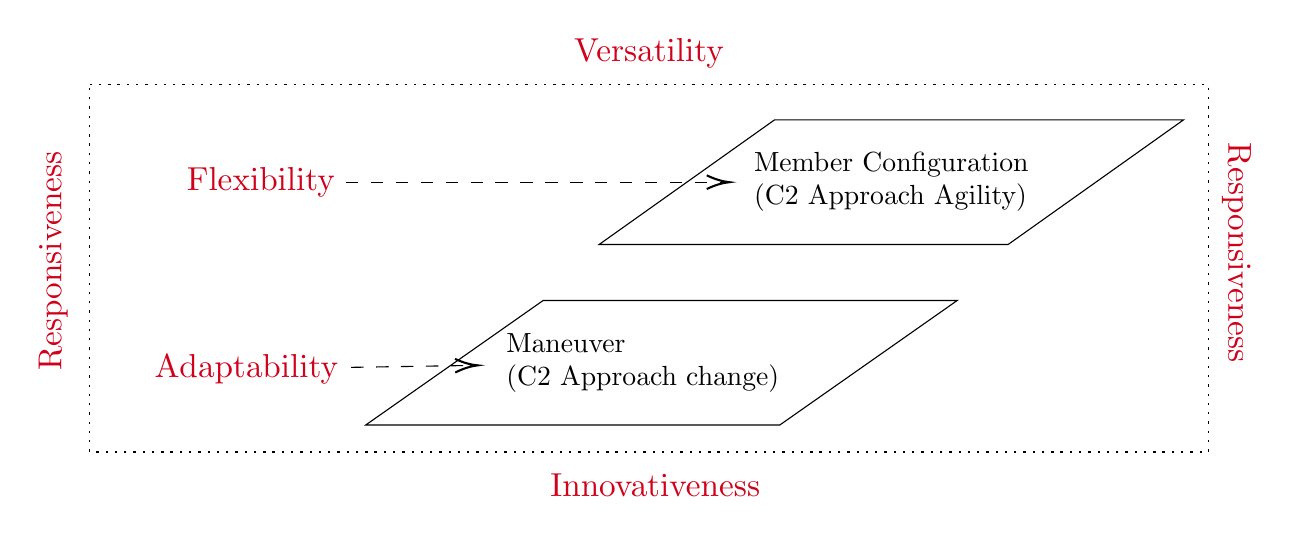
\begin{tikzpicture}[x=0.75pt,y=0.75pt,yscale=-1,xscale=1]
%uncomment if require: \path (0,300); %set diagram left start at 0, and has height of 300

%Shape: Parallelogram [id:dp7907142126701554] 
\draw   (403.45,75) -- (600.5,75) -- (516.05,135) -- (319,135) -- cycle ;
%Shape: Parallelogram [id:dp17448736771004936] 
\draw   (292,162) -- (491.5,162) -- (406,222) -- (206.5,222) -- cycle ;
%Shape: Rectangle [id:dp986244490027876] 
\draw  [dash pattern={on 0.84pt off 2.51pt}] (73.5,58) -- (612.5,58) -- (612.5,235) -- (73.5,235) -- cycle ;

% Text Node
\draw (459.75,105) node  [align=left] {Member Configuration\\(C2 Approach Agility)};
% Text Node
\draw (340,192) node  [align=left] {	Maneuver\\(C2 Approach change)};
% Text Node
\draw (343,43) node [scale=1.2,color={rgb, 255:red, 208; green, 2; blue, 27 }  ,opacity=1 ] [align=left] {Versatility};
% Text Node
\draw (346,251) node [scale=1.2,color={rgb, 255:red, 208; green, 2; blue, 27 }  ,opacity=1 ] [align=left] {Innovativeness};
% Text Node
\draw (156,105) node [scale=1.2,color={rgb, 255:red, 208; green, 2; blue, 27 }  ,opacity=1 ] [align=left] {Flexibility};
% Text Node
\draw (149,195) node [scale=1.2,color={rgb, 255:red, 208; green, 2; blue, 27 }  ,opacity=1 ] [align=left] {Adaptability};
% Text Node
\draw (626,139) node [scale=1.2,color={rgb, 255:red, 208; green, 2; blue, 27 }  ,opacity=1 ,rotate=-90] [align=left] {Responsiveness};
% Text Node
\draw (56,143) node [scale=1.2,color={rgb, 255:red, 208; green, 2; blue, 27 }  ,opacity=1 ,rotate=-270] [align=left] {Responsiveness};
% Connection
\draw  [dash pattern={on 4.5pt off 4.5pt}]  (199.5,194.21) -- (258.5,193.28) ;
\draw [shift={(260.5,193.25)}, rotate = 539.1] [color={rgb, 255:red, 0; green, 0; blue, 0 }  ][line width=0.75]    (10.93,-3.29) .. controls (6.95,-1.4) and (3.31,-0.3) .. (0,0) .. controls (3.31,0.3) and (6.95,1.4) .. (10.93,3.29)   ;

% Connection
\draw  [dash pattern={on 4.5pt off 4.5pt}]  (197,105) -- (379.75,105) ;
\draw [shift={(381.75,105)}, rotate = 180] [color={rgb, 255:red, 0; green, 0; blue, 0 }  ][line width=0.75]    (10.93,-3.29) .. controls (6.95,-1.4) and (3.31,-0.3) .. (0,0) .. controls (3.31,0.3) and (6.95,1.4) .. (10.93,3.29)   ;


\end{tikzpicture}